\chapter{Cascade of regulation - The Langevin equation}

\section{Model circuit for the cascade}
The calculations shown in this chapter are based in the work of J. M. Pedraza and A. van Oudenaarden \cite{pedraza05}. 

We will consider a set of genes whose interactions are shown on figure \ref{fig:lan-circuit} considering both intrinsic and extrinsic sources of noise. The intrinsic part refers to the inherent noise due to the low number of molecules and the nature of the reactions. This was the only source of noise consider on the previous chapter. The extrinsic part arises from another factors, such as environmental fluctuations or variations in intracellular concentrations due to sudden changes on cell volume. These factors causes fluctuations in every component of the cell and thus extrinsic noise is correlated among the different genes, while intrinsic noise is not \cite{elowitz02}.

\todo[inline]{Explain intrinsic/extrinsic noise in a section on concepts.}

\begin{figure}[H]
  \centering
  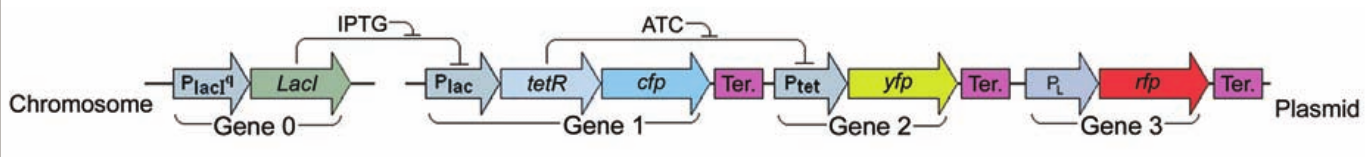
\includegraphics[width=15cm]{lan-circuit}
  \caption[Circuit used for the Langevin model]{\label{fig:lan-circuit} Circuit used in the Langevin model (from \cite{pedraza05}).}
\end{figure}

\section{Mathematical derivations}

The differential equation for the mRNA will not be considered, we will write the equation for the proteins and include the effect of mRNA in the rate of creation $k$. The results of the previous chapter for the noise in proteins caused by mRNA will also be considered. The deterministic equation for the number of proteins of gene $0$ is 

\begin{equation}
\label{eq:detgene0}
\dot{x_0}(t) = k - \gamma x_0(t).
\end{equation}

Where now $k$ represents the average number of proteins created per unit time. \footnote{For a better understanding of this point. If we assume $\gamma_r\ll\gamma_p$, we can treat the mRNA in steady state, hence eq. \eqref{eq:mas-simple_det_2} becomes eq. \eqref{eq:detgene0} with $k \coloneqq k_p\langle n_1\rangle_s =  \frac{k_pk_r}{\gamma_r} = k_rb$.}In this approach we add noise terms to the previous equation, one representing the intrinsic noise $\mu_0(t)$ and other representing the global noise $\xi_0(t)$. Hence, the equation for the stochastic process $x_0(t)$ is

\begin{equation}
\label{eq:gene0}
\dot{x_0}(t) = k - \gamma x_0(t) + \mu_0(t) + \xi_0(t).
\end{equation}

Now the quantities are taken to be stochastic processes. To find the correlations and the coefficient of variation, we need some information about the noise terms. First, the average of proteins $\langle x_0 \rangle (t)$ should follow the deterministic equation \eqref{eq:detgene0}, therefore

\begin{equation*}
\langle\mu_0\rangle(t) = \langle\xi_0\rangle(t) = 0.
\end{equation*}

Second, we will assume white noise statistics for both sources, that is, the values of the noise terms at different times are uncorrelated. Then

\begin{align}
\langle\mu_0(t)\mu_0(t+\tau)\rangle&=2\gamma(b_0+1)\bar{x}_0\delta(\tau),\label{eq:corin0}\\
\langle\xi_0(t)\xi_0(t+\tau)\rangle&=2\gamma\eta_G^2\bar{x}_0^2\delta(\tau). \label{eq:corex0}
\end{align}

\todo[inline]{Understand and explain more the constants and the assumption of white noise}

where $\eta_G$ is the strenght of the global noise, a parameter that is measured experimentally, and $b_0$ is the average number of protein produced per mRNA. In this section the bar denotes steady state average. Also, since both sources of noise are uncorrelated

\begin{equation}
\label{eq:corinex0}
\langle\mu_0(t)\xi_0(t+\tau)\rangle = 0.
\end{equation}

Define $\delta x_0 \coloneqq x_0 - \bar{x}_0$, replacing this on eq. \eqref{eq:gene0} we get

\begin{equation}
\frac{\mathrm{d}}{\mathrm{d}t}\left(\delta x_0(t) + \bar{x}_0\right) = k - \gamma (\delta x_0(t) + \bar{x}_0) + \mu_0(t) + \xi_0(t),
\end{equation}

Using the fact that $\bar{x}_0=k/\gamma$ we get

\begin{equation}
\label{eq:dgene0}
\dot{\delta x_0}(t) = -\gamma \delta x_0(t) + \mu_0(t) + \xi_0(t).
\end{equation}

We will Fourier transform the equation, find its square norm and use the Wiener-Khinchin theorem (eq. \eqref{eq:con-wkth}) to find the autocorrelations in terms of the power spectrum and to write the power spectrum of $\mu(t)$ and $\xi(t)$ in terms of their autocorrelations.

Taking the Fourier transform of eq. \eqref{eq:dgene0} and recalling that $[\mathscr{F}(\frac{\mathrm{d}x(t)}{\mathrm{d}t})](\omega) = i\omega \mathscr{F}(x(t))(\omega)$ for a function of time $x(t)$, we obtain after solving for $\hat{\delta x_0}$

\begin{equation}
\label{eq:fgene0}
\hat{\delta x_0}(\omega) = \frac{\hat{\mu_0}+\hat{\xi_0}}{\gamma + i\omega}.
\end{equation}

Taking the square norm and averaging we get

\begin{equation}
\left\langle |\hat{\delta x_0}|^2 \right\rangle = \frac{\left\langle|\hat{\mu_0}|^2\right\rangle + \left\langle\hat{\mu_0}^*\hat{\xi_0}\right\rangle+\left\langle\hat{\mu_0}\hat{\xi_0}^*\right\rangle+\left\langle|\hat{\xi_0}|^2\right\rangle}{\gamma^2 + \omega^2},
\end{equation}

And using the Wiener-Khinchin theorem and eqs. \eqref{eq:corin0} - \eqref{eq:corinex0}

\todo[inline]{Explain with more detail here}

\begin{equation}
  \label{eq:pgene0}
  \begin{split}
    \left\langle |\hat{\delta x_0}|^2 \right\rangle &= \frac{\left(2\gamma(b_0+1)\bar{x_0}+ 2\gamma\eta_G^2\bar{x_0}^2\right)\mathscr{F}(\delta(t))}{\gamma^2+\omega^2}\\
    &=\frac{2\gamma\bar{x_0}^2\left(\nicefrac{(b_0+1)}{\bar{x_0}}+ \eta_G^2\right)}{\gamma^2+\omega^2},
  \end{split}
\end{equation}

where the cross terms are zero by eq. \eqref{eq:corinex0}. Applying the inverse Fourier transform at $t=0$ we get

\begin{equation*}
\langle \delta x_0^2 \rangle = 2\gamma\bar{x_0}^2\left(\nicefrac{(b_0+1)}{\bar{x_0}}+ \eta_G^2\right)\frac{1}{2\pi}\int_{-\infty}^{\infty}\frac{d\omega}{\omega^2+\gamma^2}
\end{equation*}

The integral can be easily solved by residues resulting in $\pi/\gamma$, therefore

\begin{equation*}
\langle \delta x_0^2 \rangle = \bar{x_0}^2\left(\frac{(b_0+1)}{\bar{x_0}}+ \eta_G^2\right)
\end{equation*}

And dividing by $\bar{x_0}^2$, we obtain the coefficient of variation

\begin{equation}
  \label{eq:etagene0}
  \boxed{\eta_0^2 = \frac{(b_0+1)}{\bar{x_0}}+ \eta_G^2 = \eta_{0\text{int}}^2+\eta_G^2}.
\end{equation}

This approach enabled us to explicitly separate the total noise of gene $0$ in the intrinsic and the extrinsic part. Now we will make the calculation for gene $1$, which follows the equation.

\begin{equation}
\label{eq:gene1}
\dot{x_1}(t) = k_1(x_{0A})-\gamma x_1+\mu_1+\xi_1
\end{equation}

The decay rate $\gamma$ is the same for gene $1$ than for gene $0$ after making the assumption that the decay depends only on dilution due to cellular growth. The creation rate $k_1$ is a Hill equation for activation. The statistics for the noise terms are analogous to eqs. \eqref{eq:corin0} - \eqref{eq:corinex0}. We also need to know in this case the correlations between the noise terms corresponding to gene $0$ and the ones corresponding to gene $1$. As we have said, extrinsic sources of noise are uncorrelated

\todo[inline]{Explain more about the dilution, perhaps before}

\begin{equation}
\label{eq:corcross01}
\langle\mu_0(t)\mu_1(t+\tau)\rangle = \langle\mu_0(t)\xi_1(t+\tau)\rangle = \langle\mu_1(t)\xi_0(t+\tau)\rangle = 0,
\end{equation}

but the extrinsic parts of the noise of genes $0$ and $1$ are correlated. In analogy with eq. \eqref{eq:corex0} we get

\begin{equation}
  \langle\xi_0(t)\xi_1(t+\tau)\rangle = 2\gamma\eta_G^2\bar{x_0}\bar{x_1}\delta(\tau).
\end{equation}

\todo[inline]{Also, understand and explain the q term here}

We proceed in a similar way to gene $0$. Defining $\delta x_1(t) \coloneqq x_1(t) - \bar{x_1}$, writing eq. \eqref{eq:gene1} in terms of $\delta x_1$, $\delta x_{0A}$, and making a Taylor expansion of $f_1$ to first order in $x_{0A}$ about $\bar{x}_{0A}$ we obtain.

\begin{equation}
\dot{\delta x_1} = k_1(\bar{x_{0A}}) + \left.\frac{dk_1(x_{0A})}{dx_{0A}}\right|_{\bar{x_{0A}}}\delta x_{0A} - \gamma(\delta x_1 + \bar{x_1}) + \mu_1 + \xi_1,
\end{equation}

but from eq. \eqref{eq:gene1} we can see that $\bar{x_1} = \nicefrac{k_1(\bar{x_{0A}})}{\gamma}$, therefore

\begin{equation}
  \label{eq:dgene1}
  \dot{\delta{x_1}(t)}=c_1\delta x_{0A}-\gamma\delta x_1 + \mu_1 \xi_1,
\end{equation}

where $c_1 \coloneqq \left.\nicefrac{dk_1(x_{0A})}{dx_{0A}}\right|_{\bar{x_{0A}}}$ Fourier transforming and solving for $\hat{\delta x_1}$ we get

\begin{equation*}
  \hat{\delta x_1}=\frac{c_1\hat{\delta x_{0A}}+\hat{\mu_1}+\hat{\xi_1}}{\gamma + i\omega}.
\end{equation*}

Taking the square norm and averaging

\begin{equation*}
  \label{eq:pgene1}
  \begin{split}
    \left\langle|\hat{\delta x_1}|^2\right\rangle &= \frac{1}{\omega^2+\gamma^2}\left(c_1\hat{\delta x_{0A}} + \hat{\mu_1} + \hat{\xi_1}\right)\left(c_1\hat{\delta x_{0A}}^* + \hat{\mu_1}^* + \hat{\xi_1}^*\right)\\
    &=\frac{1}{\omega^2+\gamma^2}\left(c_1^2 \left\langle|\hat{\delta x_{0A}}|^2\right\rangle + c_1\left(\langle\hat{\delta x_{0A}}\hat{\xi_1}^*\rangle+\langle\hat{\delta x_{0A}}^*\hat{\xi_1}\rangle\right) +  \left\langle|\hat{\mu_1}|^2\right\rangle +  \left\langle|\hat{\xi_1}|^2\right\rangle\right)
  \end{split}
\end{equation*}

Using the Wiener-Khinchin theorem and the equations for the correlations we get

\begin{align*}
  \left\langle|\hat{\mu_1}|^2\right\rangle &= 2\gamma(b_1+1)\bar{x_1},\\
  \left\langle|\hat{\xi_1}|^2\right\rangle &= 2\gamma\eta_G^2\bar{x_1}^2,
\end{align*}

since the Fourier transform of the Dirac delta is $1$. Also, from eqs. \eqref{eq:fgene0} and \eqref{eq:pgene0} we get

\begin{align*}
\left\langle|\hat{\delta x_{0A}}|^2\right\rangle &= \frac{2\gamma\bar{x_0}^2\left(\nicefrac{(b_0+1)}{\bar{x_0}}+ \eta_G^2\right)}{\gamma^2+\omega^2},\\
\langle\hat{\delta x_{0A}}\hat{\xi_1}^*\rangle &= \frac{1}{\gamma+i\omega}\left(\langle\hat{\mu_0}\hat{\xi_1}^*\rangle + \langle\hat{\xi_0}\hat{\xi_1}^*\rangle \right) = \frac{\langle\hat{\xi_0}\hat{\xi_1}^*\rangle}{\gamma+i\omega}\\
\langle\hat{\delta x_{0A}}^*\hat{\xi_1}\rangle &= \frac{1}{\gamma-i\omega}\left(\langle\hat{\mu_0}^*\hat{\xi_1}\rangle + \langle\hat{\xi_0}^*\hat{\xi_1}^*\rangle \right) = \frac{\langle\hat{\xi_0}^*\hat{\xi_1}\rangle}{\gamma-i\omega}
\end{align*}

Where the last step in the last two equations comes from the Wiener-Khinchin theorem and eq. \eqref{eq:corcross01}. Replacing the previous equations in eq. \eqref{eq:pgene1} and taking the inverse transform we get for the variance

\begin{equation}
  \begin{split}
    \langle \delta x_1^2\rangle &= 2\gamma\bar{x_0}^2c_1^2\left(\nicefrac{(b_0+1)}{\bar{x_0}}+ \eta_G^2\right)\frac{1}{2\pi}\int_{-\infty}^{\infty}\frac{d\omega}{(\omega^2+\gamma^2)^2}\\
    &+2\gamma\eta_G^2\bar{x_0}\bar{x_1}c_1\frac{1}{2\pi}\left(\int_{-\infty}^{\infty}\frac{d\omega}{(\gamma + i\omega)(\omega^2+\gamma^2)} + \int_{-\infty}^{\infty}\frac{d\omega}{(\gamma - i\omega)(\omega^2+\gamma^2)}\right)\\
    &+2\gamma\bar{x_1}^2 \left(\nicefrac{(b_1+1)}{\bar{x_1}}+\eta_G^2\right)\frac{1}{2\pi}\int_{-\infty}^{\infty}\frac{d\omega}{\omega^2+\gamma^2}.
  \end{split}
\end{equation} 

Solving the integrals in the complex plane and rearranging

\begin{equation}
  \langle \delta x_1^2\rangle = \frac{c_1^2\bar{x_0}^2}{2\gamma^2}\left(\nicefrac{(b_0+1)}{\bar{x_0}}+ \eta_G^2\right) + \frac{c_1\eta_G^2\bar{x_0}\bar{x_1}}{\gamma} + \bar{x_1}^2\left(\nicefrac{(b_1+1)}{\bar{x_1}}+\eta_G^2\right).
\end{equation}

Writing in terms of the logarithmic gain $H_{ji}\coloneqq -\frac{\langle x_i\rangle}{\langle x_j\rangle}\frac{1}{\gamma_j}\frac{\mathrm{d} f_j(x_i)}{\mathrm{d}x_i}$, in this case it becomes $H_{10}=-\frac{c_1\bar{x_0}}{\gamma x_1}$. Dividing by $\bar{x_1}^2$ and rearranging

\begin{equation}
  \label{eq:etagene1}
  \boxed{\eta_1^2 = \eta_{1\text{int}}^2 + \frac{1}{2}H_{10}^2\eta_0^2+\eta_G^2\left(1-H_{10}\right)}.
\end{equation}

\todo[inline]{TODO: Explain a lot more about the logarithmic gain}

Where $\eta_{1\text{int}}^2 = \nicefrac{(b_1+1)}{\bar{x_1}}$ and $\eta_0^2$ is given by eq. \ref{eq:etagene0}.

The result can be interpreted as follows, the total noise in gene one is given by the intrinsic part, the noise from gene $0$ that is propagated to gene $1$ (including both its intrinsic and global part) and the global noise that enters directly into gene $1$. The factor of $1/2$ arises from the time averaging since we assumed equal degradation rates for both proteins.

\todo[inline]{See if it is better to do it with different gammas}

For gene $2$ we proceed similarly, with analogous statistics for the noise terms, the resulting noise is

\begin{equation}
  \label{eq:etagene2}
  \boxed{\eta_2^2 = \eta_{2\text{int}}^2 + \frac{1}{2}H_{21}^2\eta_1^2+\frac{1}{8}H_{21}^2H_{10}^2\eta_0^2+\eta_G^2\left(1-H_{21}-\frac{1}{4}H_{21}^2H_{10}+\frac{1}{2}H_{21}H_{10}\right)}.
\end{equation}

Which contains the intrinsic noise of gene $2$, the contribution from the total noise of gene $1$, the contribution from the total noise of gene $0$ that is transmitted first to gene $1$ and then to gene $2$ and the global noise that enters directly. 

The correlations can be found in a similar fashion.

\todo[inline]{TODO: Find the correlations and do the analysis that JM did on SysBio class}

\section{Explicit expressions for the logarithmic gain}



\section{Analysis and implications}

As it can be noticed in eqs. \eqref{eq:etagene0}, \eqref{eq:etagene1} and \eqref{eq:etagene2}, the noise propagation follows the sequence of fig. \ref{fig:lan-noise_sources}. For each gene there is an independent intrinsic noise a correlated global noise, and both the transmitted global and intrinsic noise between the genes of the cascade whose strenght is determined by the logarithmic gain $H$.

\begin{figure}[H]
  \centering
  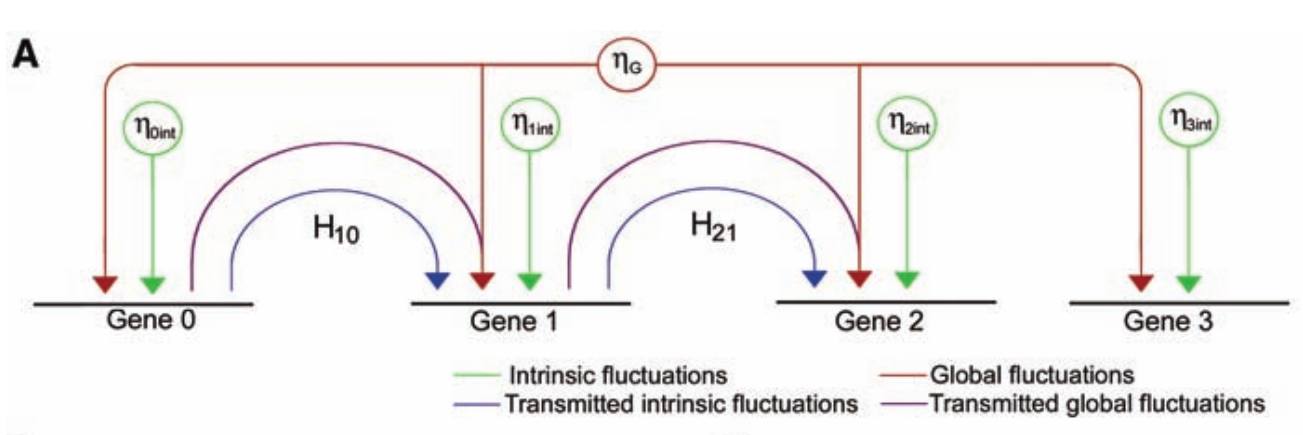
\includegraphics[width=15cm]{lan-noise_sources}
  \caption[Propagation of noise through a cascade]{\label{fig:lan-noise_sources} Different sources of noise and their propagation along the cascade of regulation (from \cite{pedraza05}).}
\end{figure}

\todo[inline]{TODO: Analyze the results physically (recall SysBio class), reproduce the graphics and analyze them}

This approach enables us to calculate the coefficient of variation for a cascade of regulation and separate the different sources of noise. Also, it enables to write the effect of the upstream genes in terms of the logarithmic gain, making it very intuitive. The results of the theoretical model were tested with experiments where the genes that are part of the cascade are transcribed bicistronicaly with fluorescent reporters. The fluctuations in the intensity of the reporters was used to measure the noise in the population of cells.
